\documentclass[11pt,letterpaper]{article}
\usepackage[margin=1in]{geometry}
\usepackage[T1]{fontenc}
\usepackage{lmodern}
\usepackage{amsmath,amssymb,graphicx,booktabs,tabularx,float,caption}
\usepackage[hidelinks]{hyperref}
\urlstyle{same}
\captionsetup{font=small,labelfont=bf}
\setlength{\parskip}{0.35em}
\setlength{\parindent}{0pt}
\setlength{\tabcolsep}{5pt}
\renewcommand{\arraystretch}{1.12}
\setlength{\textfloatsep}{12pt plus 2pt minus 2pt}
\setlength{\intextsep}{12pt plus 2pt minus 2pt}
\emergencystretch=1em
\clubpenalty=10000
\widowpenalty=10000
\brokenpenalty=10000
\raggedbottom
\title{BIOSTAT825 Homework 1\\Bandit Experiments}
\author{Zhouhan Qian}
\hypersetup{pdfauthor={Zhouhan Qian}}
\date{}
\begin{document}
\maketitle
\vspace{-2em}

\section*{Experimental setup}
All experiments used $T=1000$ rounds. The number of runs was $N=50$ for Parts 1--2,
$N=5$ for Parts 3--4, $N=10$ for Parts 5--6, and $N=3$ per role or profile for Parts 7A--7B.
Each run started with fresh policy state. Within each comparison, the methods received
matched environment randomness. Policy randomness was kept separate from environment randomness.

Parts 1--6 measured cumulative pseudo-regret,
\[
 R_T=\sum_{t=1}^{T}\left[\max_a\mu_t(a)-\mu_t(a_t)\right],
\]
where $\mu_t(a)$ is the expected reward of arm $a$. Lower regret is better.
Parts 7A--7B instead measured cumulative sampled reward, $C_T=\sum_{t=1}^{T}r_t$, where higher is better.
Tables give means and sample standard deviations across runs. Shading in the plots
shows pointwise empirical 10th--90th percentiles, not confidence intervals.
The comparisons describe the fixed environments, candidate sets, and seeds used here;
this is particularly limiting for the three-run LLM experiments.

\section*{Part 1. Linear contextual bandits}
\pdfbookmark[1]{Part 1. Linear contextual bandits}{part1}
The linear environment used $d=7$, three arms per round, and two fixed context sets.
The arm vectors and unknown coefficient $\theta$ had unit norm. Rewards were
$x^\top\theta+\varepsilon$, with $\varepsilon\sim N(0,1)$.
Greedy and $\epsilon$-greedy used $\epsilon=0$ and $0.1$, respectively.
LinTS used a zero-mean Gaussian prior with precision one and unit noise variance.
LinUCB used $\lambda=\alpha=1$ and $\delta=0.2$, with the supplied exploration radius.

Greedy had the lowest mean regret, but its results varied widely. Its median was 3.23, while its worst run reached 237.06. The low mean therefore hides an occasional poor run.

LinTS had lower mean regret than LinUCB, whereas LinUCB had the smallest standard deviation. $\epsilon$-greedy had the highest mean regret among the four methods. Its continued random exploration is consistent with this result, since some random choices remain costly after useful estimates have been learned.

\begin{table}[H]
\centering
\small
\caption{Final cumulative regret in the linear environment ($N=50$).}
\label{tab:part1}
\begin{tabularx}{\linewidth}{@{}Xr@{}}
\toprule
Method & Final cumulative regret \\
\midrule
Greedy & 11.43 $\pm$ 34.59 \\
$\epsilon$-greedy, $\epsilon=0.1$ & 66.45 $\pm$ 28.18 \\
LinUCB & 42.52 $\pm$ 11.60 \\
LinTS & 34.95 $\pm$ 14.39 \\
\bottomrule
\end{tabularx}
\end{table}

\begin{figure}[H]
\centering
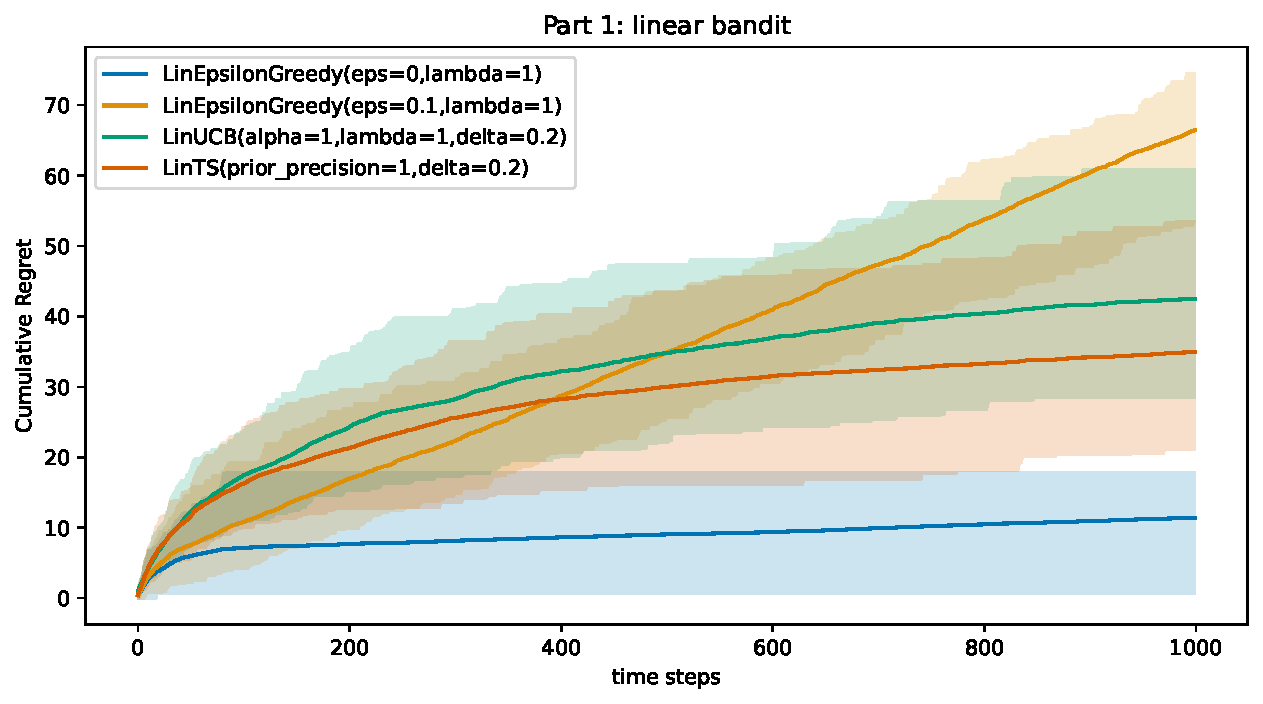
\includegraphics[width=0.96\linewidth]{../artifacts/full-20261101-1923/parts1-6/figures/cell_008_figure_001.pdf}
\caption{Cumulative regret for the four linear policies.}
\label{fig:part1}
\end{figure}

\section*{Part 2. Choosing the exploration rule for $\epsilon$-LinTS}
\pdfbookmark[1]{Part 2. Choosing the exploration rule for epsilon-LinTS}{part2}
At round $t$, $\epsilon$-LinTS used Thompson sampling with probability $\epsilon_t$
and the greedy ridge prediction otherwise. The tested choices were $0.05$, $1/d=1/7$,
$1/t$, and an additional constant $0.2$. The $1/t$ schedule started at one.
The sweep used trajectory seed 62 in the Part 1 environment.

The sweep selected $\epsilon_t=1/t$ because it had the lowest mean regret, 14.93. However, its standard deviation was 58.04. The 1/d rule had a slightly higher mean of 18.56 and a much smaller standard deviation of 12.84.

\begin{table}[H]
\centering
\small
\caption{Exploration-rule sweep for $\epsilon$-LinTS ($N=50$).}
\label{tab:epsilon}
\begin{tabularx}{\linewidth}{@{}Xr@{}}
\toprule
$\epsilon$-LinTS rule & Sweep regret (seed 62) \\
\midrule
0.05 & 19.57 $\pm$ 32.78 \\
1/d = 1/7 & 18.56 $\pm$ 12.84 \\
1/t & 14.93 $\pm$ 58.04 \\
0.2 (additional choice) & 23.02 $\pm$ 21.77 \\
\bottomrule
\end{tabularx}
\end{table}

\begin{figure}[H]
\centering
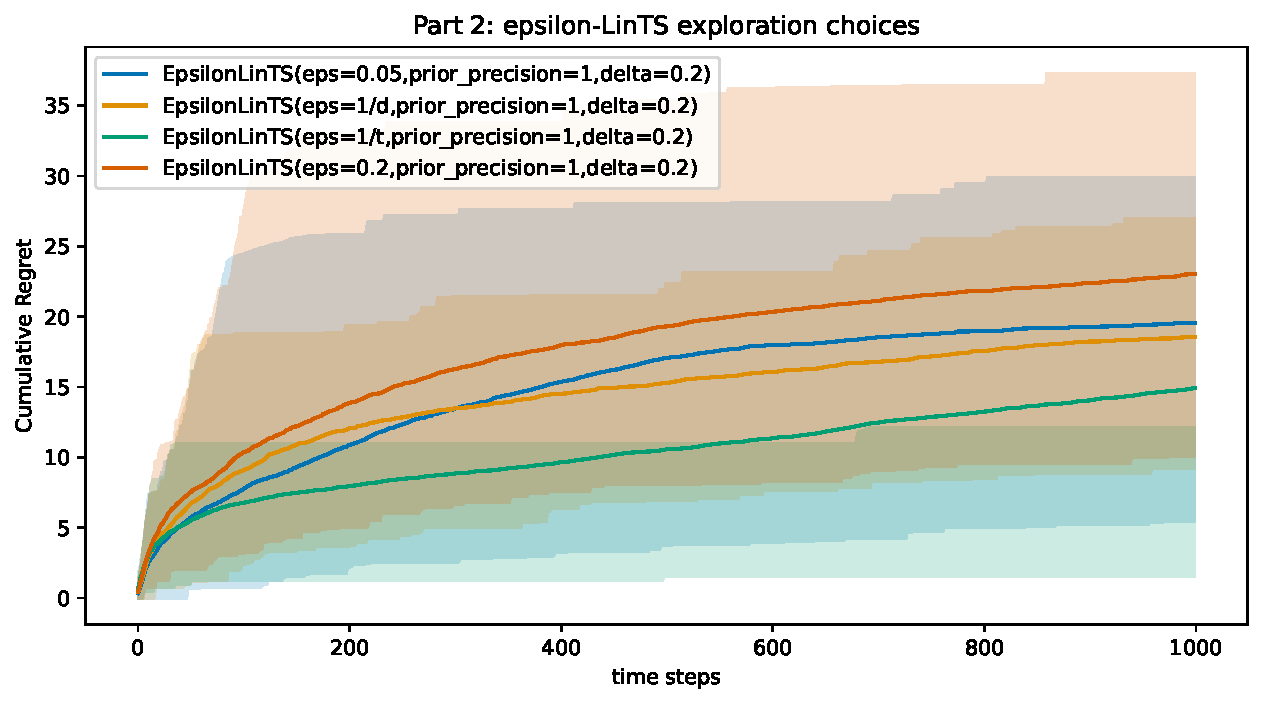
\includegraphics[width=0.96\linewidth]{../artifacts/full-20261101-1923/parts1-6/figures/cell_012_figure_002.pdf}
\caption{Cumulative regret in the exploration-rule sweep.}
\label{fig:epsilon}
\end{figure}

The rule with the lowest sweep mean was then compared with fresh baseline agents,
using trajectory seed 63. Table~\ref{tab:part2} and Figure~\ref{fig:part2}
show this second comparison.

In the fresh comparison, the selected rule had lower mean regret than $\epsilon$-greedy, LinUCB, and LinTS, but Greedy remained lower. Its median was 4.18, yet two runs exceeded 200 and the maximum reached 385.11. These poor runs raised the mean and explain the large standard deviation. They can also place the mean above the 90th percentile. Selecting 1/t by its sweep mean therefore did not make it a reliable choice in every run. The steadier 1/d results also deserve attention when choosing an exploration rule.

\begin{table}[H]
\centering
\small
\caption{Fresh comparison using the selected $1/t$ rule ($N=50$).}
\label{tab:part2}
\begin{tabularx}{\linewidth}{@{}Xr@{}}
\toprule
Method & Final cumulative regret \\
\midrule
Greedy & 9.87 $\pm$ 33.30 \\
$\epsilon$-greedy, $\epsilon=0.1$ & 63.19 $\pm$ 11.99 \\
LinTS & 32.26 $\pm$ 10.34 \\
LinUCB & 45.26 $\pm$ 13.26 \\
Selected $\epsilon$-LinTS, 1/t & 18.61 $\pm$ 62.81 \\
\bottomrule
\end{tabularx}
\end{table}

\begin{figure}[H]
\centering
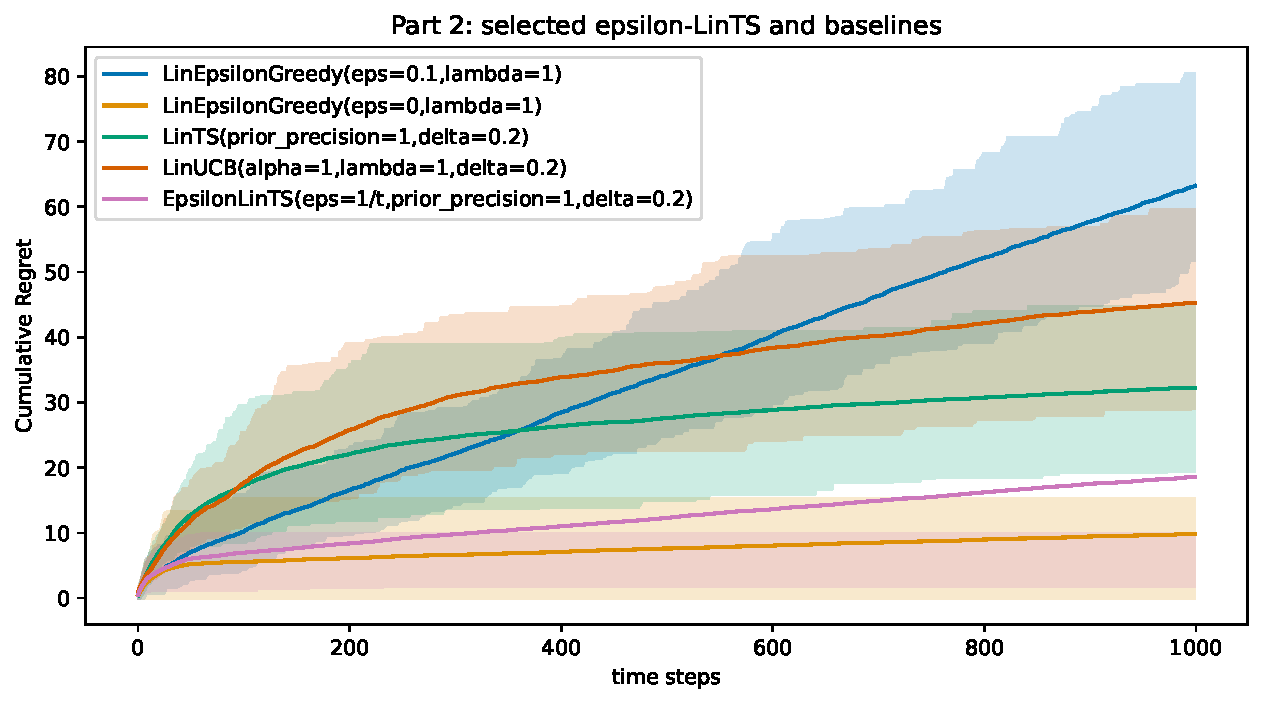
\includegraphics[width=0.96\linewidth]{../artifacts/full-20261101-1923/parts1-6/figures/cell_012_figure_003.pdf}
\caption{Selected $\epsilon$-LinTS compared with the required baselines and Greedy.}
\label{fig:part2}
\end{figure}

\section*{Part 3. Linear-model LMCTS}
\pdfbookmark[1]{Part 3. Linear-model LMCTS}{part3}
LMCTS selected the arm with the largest prediction from its current noisy parameter iterate.
After each observation, the bias-free linear model received one warm-start Langevin update
using the complete observation history. With mean squared error $L(\theta)$, the update was
\[
 \theta\leftarrow\theta-\eta\bigl(\nabla L(\theta)+\lambda\theta\bigr)
 +\sigma\sqrt{2\eta\beta^{-1}}\,z,\qquad z\sim N(0,I).
\]
The settings were $\eta=0.1$, $\beta^{-1}=0.01$, $\sigma=1$, and $\lambda=1$.
This finite-step, regularized-loss sampler was the implementation assumption used in the notebook;
it does not give an exact posterior guarantee. The comparison used a new linear environment
with environment seed 72 and trajectory seed 73.

LMCTS had the lowest mean regret, followed by LinTS and LinUCB. This result supports the chosen LMCTS settings in the new linear environment, although the comparison contains only five runs.

The epsilon rule selected in Part 2 did not transfer reliably. Its median regret was 27.88, but one run reached 319.71 and raised the mean substantially. Early estimation errors may persist when the exploration probability decreases rapidly. Direct numerical comparisons with Part 2 would also mix changes in the environment and trajectory seeds.

\begin{table}[H]
\centering
\small
\caption{Linear-model LMCTS and baselines in the new linear environment ($N=5$).}
\label{tab:part3}
\begin{tabularx}{\linewidth}{@{}Xr@{}}
\toprule
Method & Final cumulative regret \\
\midrule
LinTS & 34.54 $\pm$ 9.67 \\
LinUCB & 36.21 $\pm$ 5.79 \\
$\epsilon$-LinTS, 1/t & 80.18 $\pm$ 134.96 \\
Linear-model LMCTS & 25.82 $\pm$ 8.99 \\
\bottomrule
\end{tabularx}
\end{table}

\begin{figure}[H]
\centering
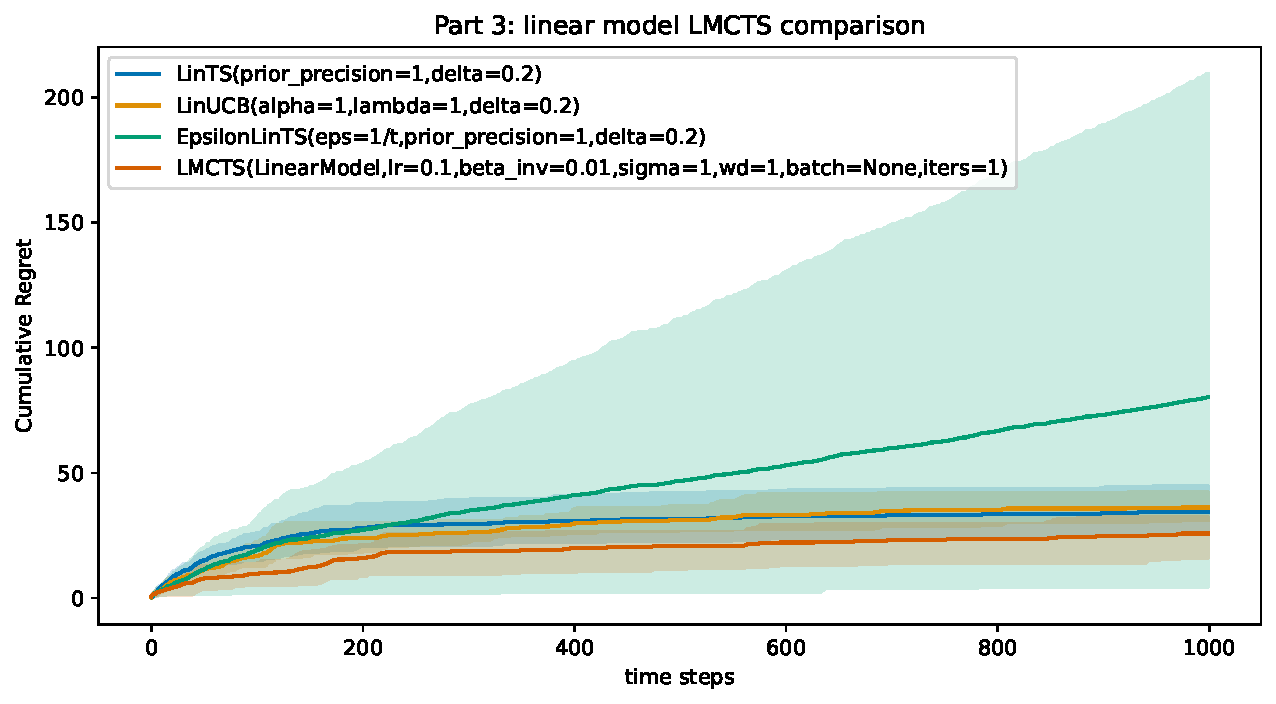
\includegraphics[width=0.96\linewidth]{../artifacts/full-20261101-1923/parts1-6/figures/cell_019_figure_004.pdf}
\caption{Cumulative regret for linear-model LMCTS and the three comparison policies.}
\label{fig:part3}
\end{figure}

\section*{Part 4. Linear, logistic, and quadratic rewards}
\pdfbookmark[1]{Part 4. Linear, logistic, and quadratic rewards}{part4}
The three environments shared the same six arm-feature vectors and coefficient.
Their expected rewards were $x^\top\theta$, $\{1+\exp(-x^\top\theta)\}^{-1}$,
and $10(x^\top\theta)^2$. Linear and quadratic observations had Gaussian noise with
standard deviation one; logistic observations were Bernoulli.
The coefficient, feature geometry, and trajectory seeds were 82, 83, and 84.
The policies used the same settings as in Part 3.

LinTS had the lowest mean regret under linear and logistic rewards. LinUCB performed much better under quadratic rewards. In that environment, LinTS varied widely, while $\epsilon$-LinTS and LMCTS accumulated much larger regret.

The nonlinear reward functions alone do not explain these differences. There are only six fixed arm vectors in seven dimensions. If those vectors are independent, a linear model can interpolate their mean rewards. Exploration, regularization, and finite-step fitting could also affect the results, and this experiment does not separate their contributions. The reward scales differ across environments, so the useful comparisons are between methods within each environment.

\begin{table}[H]
\centering
\small
\caption{Final regret under the three reward functions ($N=5$ per environment).}
\label{tab:part4}
\begin{tabularx}{\linewidth}{@{}Xrrr@{}}
\toprule
Method & Linear & Logistic & Quadratic \\
\midrule
LinTS & 39.78 $\pm$ 8.85 & 34.53 $\pm$ 6.13 & 513.62 $\pm$ 556.66 \\
LinUCB & 60.99 $\pm$ 16.04 & 45.97 $\pm$ 1.98 & 43.52 $\pm$ 17.28 \\
$\epsilon$-LinTS, 1/t & 105.17 $\pm$ 164.63 & 95.00 $\pm$ 57.11 & 1783.07 $\pm$ 547.18 \\
Linear-model LMCTS & 44.14 $\pm$ 13.88 & 43.63 $\pm$ 30.21 & 1924.01 $\pm$ 501.59 \\
\bottomrule
\end{tabularx}
\end{table}

\begin{figure}[H]
\centering
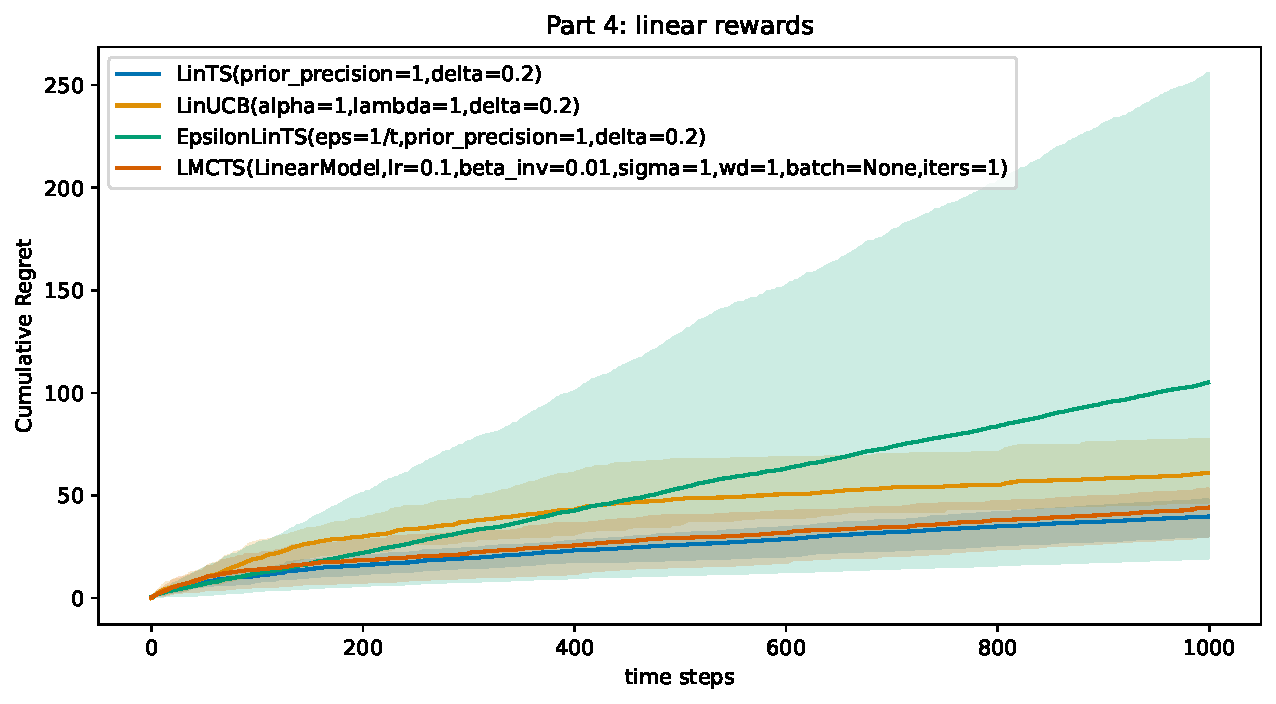
\includegraphics[width=0.96\linewidth]{../artifacts/full-20261101-1923/parts1-6/figures/cell_022_figure_005.pdf}
\caption{Cumulative regret with linear rewards and the shared arm geometry.}
\label{fig:part4-linear}
\end{figure}

\begin{figure}[H]
\centering
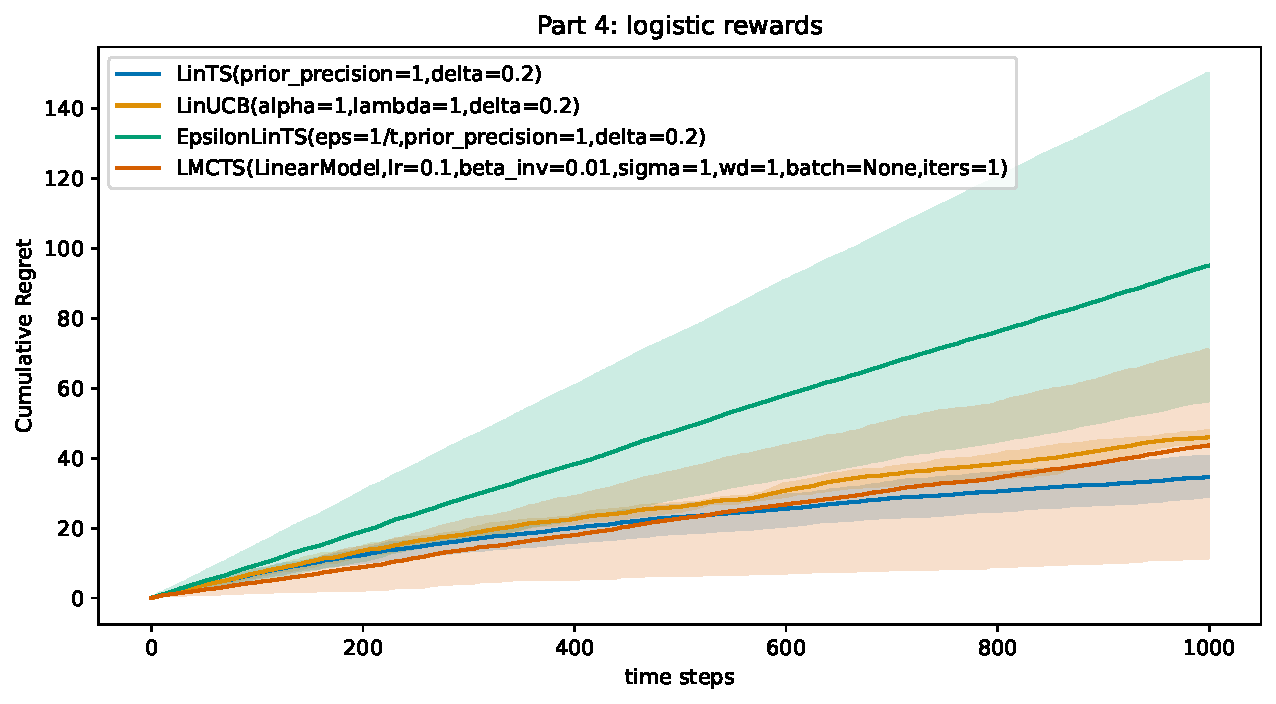
\includegraphics[width=0.96\linewidth]{../artifacts/full-20261101-1923/parts1-6/figures/cell_023_figure_006.pdf}
\caption{Cumulative regret with logistic rewards and the shared arm geometry.}
\label{fig:part4-logistic}
\end{figure}

\begin{figure}[H]
\centering
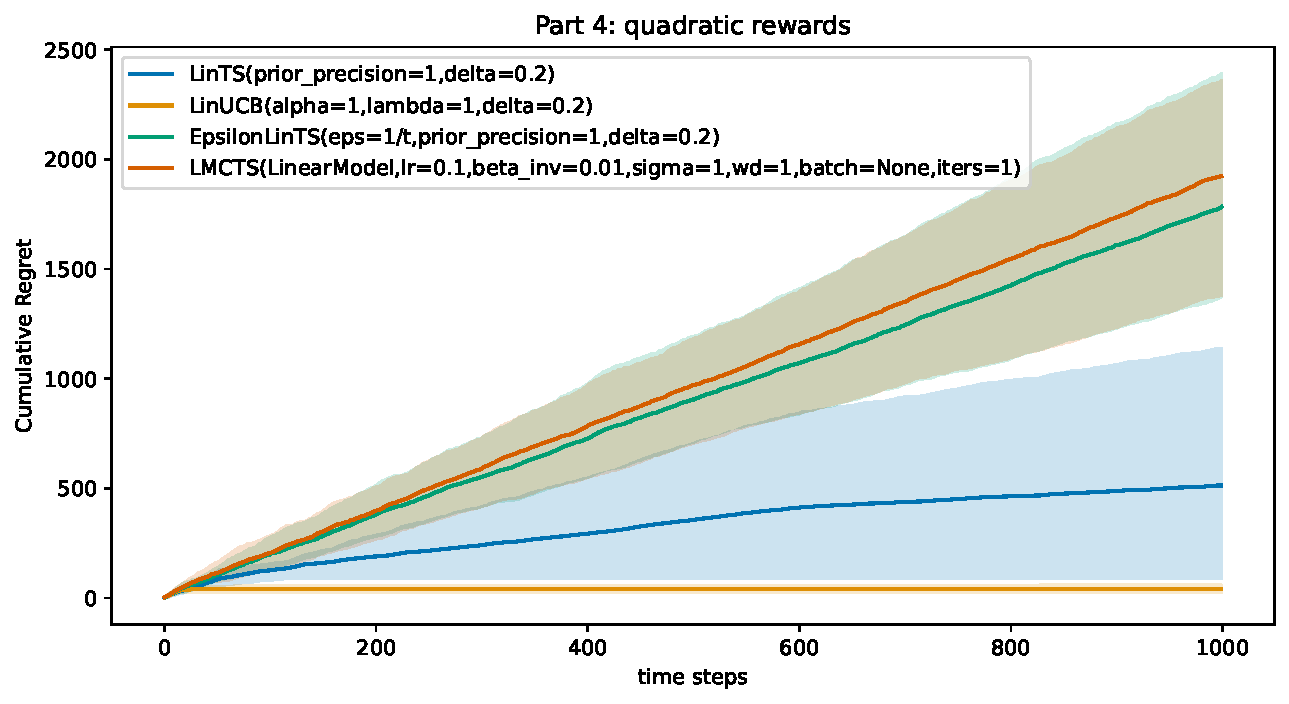
\includegraphics[width=0.96\linewidth]{../artifacts/full-20261101-1923/parts1-6/figures/cell_024_figure_007.pdf}
\caption{Cumulative regret with quadratic rewards and the shared arm geometry.}
\label{fig:part4-quadratic}
\end{figure}

\clearpage
\section*{Part 5. Neural policies in the quadratic environment}
\pdfbookmark[1]{Part 5. Neural policies in the quadratic environment}{part5}
Each policy used a separate 50-unit LeakyReLU network. Neural $\epsilon$-greedy used
$\epsilon=0.1$. NeuralTS and NeuralUCB used $\nu=\lambda=1$ and diagonal precision
$D=\lambda I+\sum_s\phi(x_s)^2$, where $\phi(x)=\nabla_\theta f_\theta(x)/\sqrt{50}$.
NeuralUCB added $\nu\sqrt{\sum_j\phi_j(x)^2/D_j}$ to its prediction;
NeuralTS shared one Gaussian parameter perturbation across the candidate arms.
These uncertainty approximations were implementation choices.

Training used five steps and batches of up to 64 observations. The non-Langevin policies
used SGD with learning rate $0.01$; NeuralTS and NeuralUCB were regularized toward initial weights.
NeuralLMCTS used learning rate $0.01$, inverse temperature $0.01$, noise multiplier one,
and decay $0.01$. The environment and trajectory seed was 505.

\begin{table}[H]
\centering
\small
\caption{Neural-policy comparison in the quadratic environment ($N=10$).}
\label{tab:part5}
\begin{tabularx}{\linewidth}{@{}Xr@{}}
\toprule
Method & Final cumulative regret \\
\midrule
Neural $\epsilon$-greedy ($\epsilon=0.1$) & 97.81 $\pm$ 55.26 \\
NeuralTS & 58.26 $\pm$ 36.98 \\
NeuralUCB & 181.78 $\pm$ 310.49 \\
NeuralLMCTS & 88.83 $\pm$ 43.57 \\
\bottomrule
\end{tabularx}
\end{table}

\begin{figure}[H]
\centering
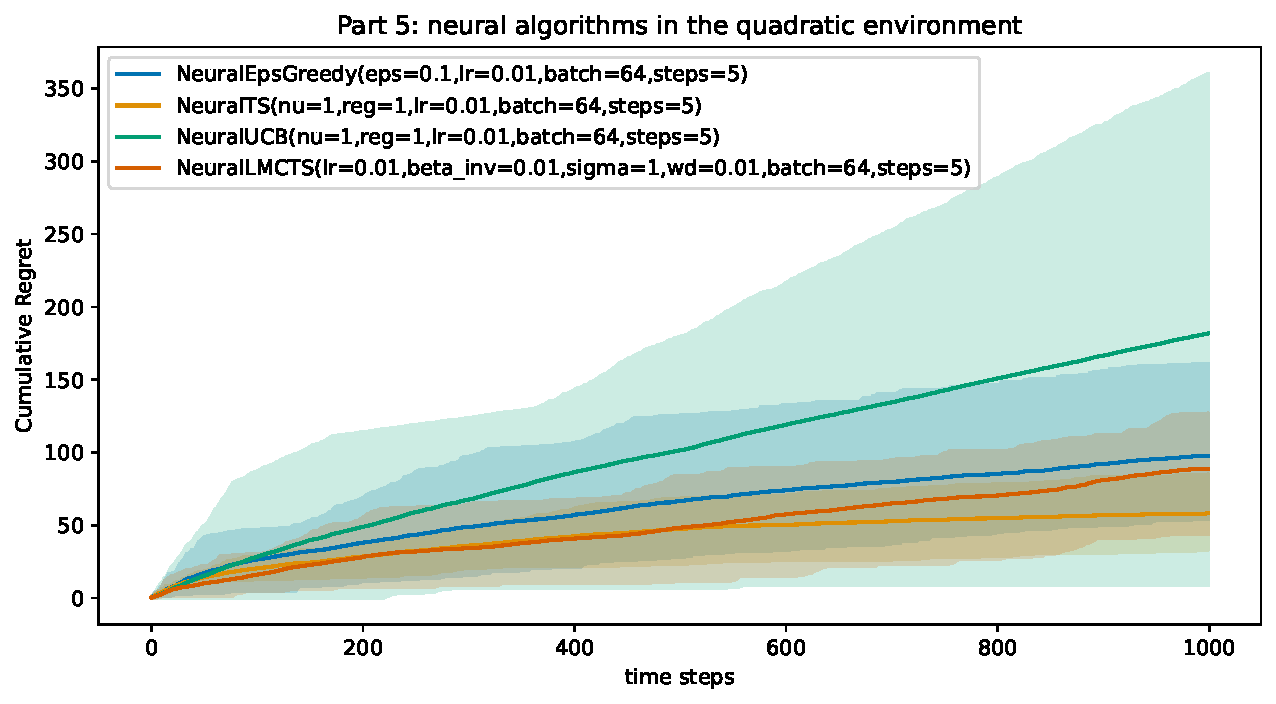
\includegraphics[width=0.96\linewidth]{../artifacts/full-20261101-1923/parts1-6/figures/cell_034_figure_008.pdf}
\caption{Cumulative regret for the neural policies in the quadratic environment.}
\label{fig:part5}
\end{figure}

NeuralTS had the lowest mean regret, followed by NeuralLMCTS and neural $\epsilon$-greedy. NeuralUCB was much less consistent. Its median was 51.58, but one run reached 1008.40, raising both the mean and standard deviation. Its high average therefore does not describe every run.

NeuralLMCTS initially performed better than NeuralTS: their mean regrets at round 100 were 16.00 and 20.38, respectively. NeuralTS later accumulated less additional regret during rounds 501-1000, at 10.67 versus 40.46. Thus, the early advantage did not persist to the final comparison. Part 5 uses a new environment generated with seed 505. Its lower regret cannot establish a controlled improvement of neural methods over the linear methods in Part 4.


\section*{Part 6. Shuttle classification and LMCTS tuning}
\pdfbookmark[1]{Part 6. Shuttle classification and LMCTS tuning}{part6}
The shuttle data were loaded through OpenML. Each row-normalized, nine-dimensional
context was placed into one of seven disjoint arm blocks, giving 63 inputs.
A correct class choice earned reward one, and an incorrect choice earned zero.
Regret therefore counted incorrect online choices.

The LMCTS sweep changed the learning rate, inverse temperature, or number of updates
one setting at a time. Width 50, batch size 64, noise multiplier one, and weight decay
$0.01$ were fixed. The tuning and fresh comparison seeds were 606 and 607.

The seed-606 sweep selected learning rate 0.01, inverse temperature 0.001, and five updates because this configuration had the lowest mean regret. Its variability was much greater than the reference setting's. Ten updates produced steadier results but did not improve the mean.

\begin{table}[H]
\centering
\small
\caption{LMCTS tuning on shuttle ($N=10$).}
\label{tab:shuttle-tuning}
\begin{tabularx}{\linewidth}{@{}Xrrrr@{}}
\toprule
Configuration & $\eta$ & $\beta^{-1}$ & Updates & Final regret \\
\midrule
Reference & 0.01 & 0.01 & 5 & 352.70 $\pm$ 47.75 \\
Lower noise & 0.01 & 0.001 & 5 & 316.90 $\pm$ 151.41 \\
Smaller step & 0.003 & 0.01 & 5 & 375.50 $\pm$ 128.20 \\
More updates & 0.01 & 0.01 & 10 & 361.10 $\pm$ 35.28 \\
\bottomrule
\end{tabularx}
\end{table}

\begin{figure}[H]
\centering
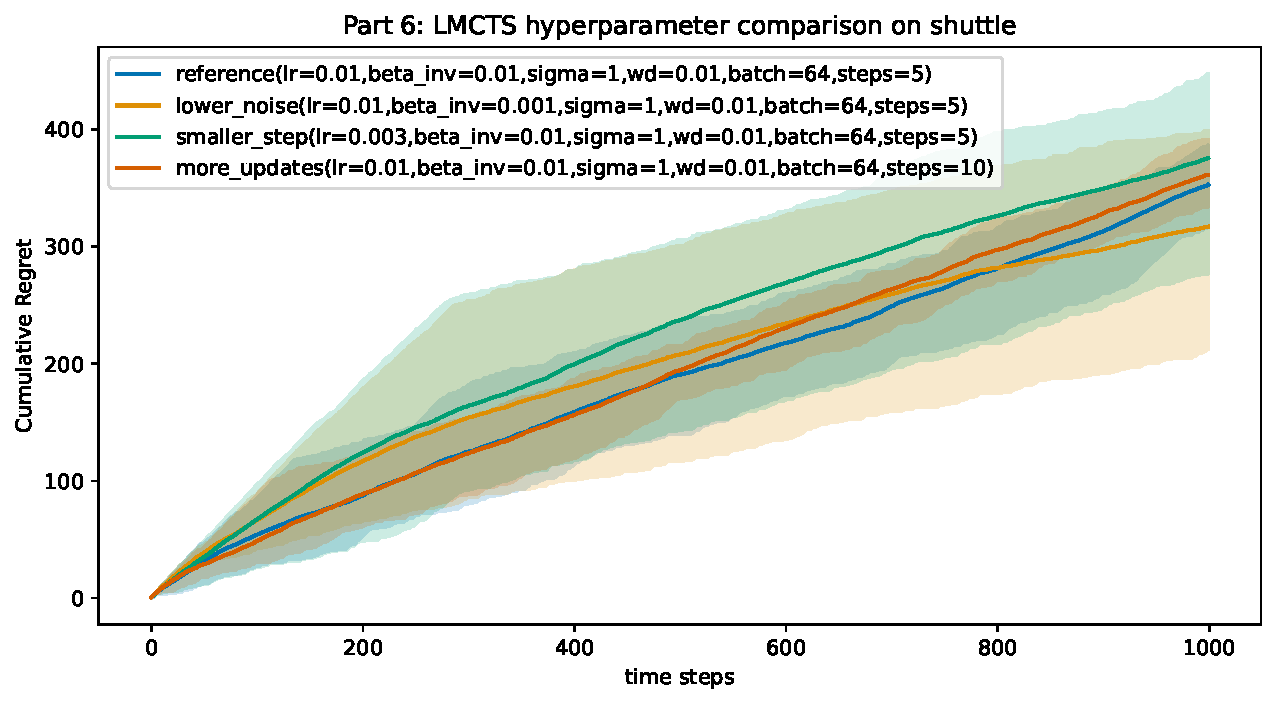
\includegraphics[width=0.96\linewidth]{../artifacts/full-20261101-1923/parts1-6/figures/cell_038_figure_009.pdf}
\caption{Cumulative regret for the four tested LMCTS configurations.}
\label{fig:shuttle-tuning}
\end{figure}

NeuralTS performed best in the fresh seed-607 comparison. The selected LMCTS setting increased from 316.90 tuning regret to 468.10, so its favorable sweep result did not transfer reliably to new trajectories. The fresh comparison does not show whether this setting is better than the other three LMCTS configurations.

For shuttle, regret counts incorrect choices. Online accuracy is therefore 1 - R(1000)/1000, rather than held-out supervised test accuracy. The large variation in LMCTS results makes repeated runs necessary when judging the selected configuration.

\begin{table}[H]
\centering
\small
\caption{Fresh shuttle comparison with the selected LMCTS setting ($N=10$).}
\label{tab:shuttle-final}
\begin{tabularx}{\linewidth}{@{}Xrr@{}}
\toprule
Method, fresh seed 607 & Final regret & Mean online accuracy \\
\midrule
Neural $\epsilon$-greedy & 364.80 $\pm$ 84.00 & 63.52\% \\
NeuralTS & 327.70 $\pm$ 51.85 & 67.23\% \\
NeuralUCB & 756.50 $\pm$ 275.05 & 24.35\% \\
Selected NeuralLMCTS & 468.10 $\pm$ 253.10 & 53.19\% \\
\bottomrule
\end{tabularx}
\end{table}

\begin{figure}[H]
\centering
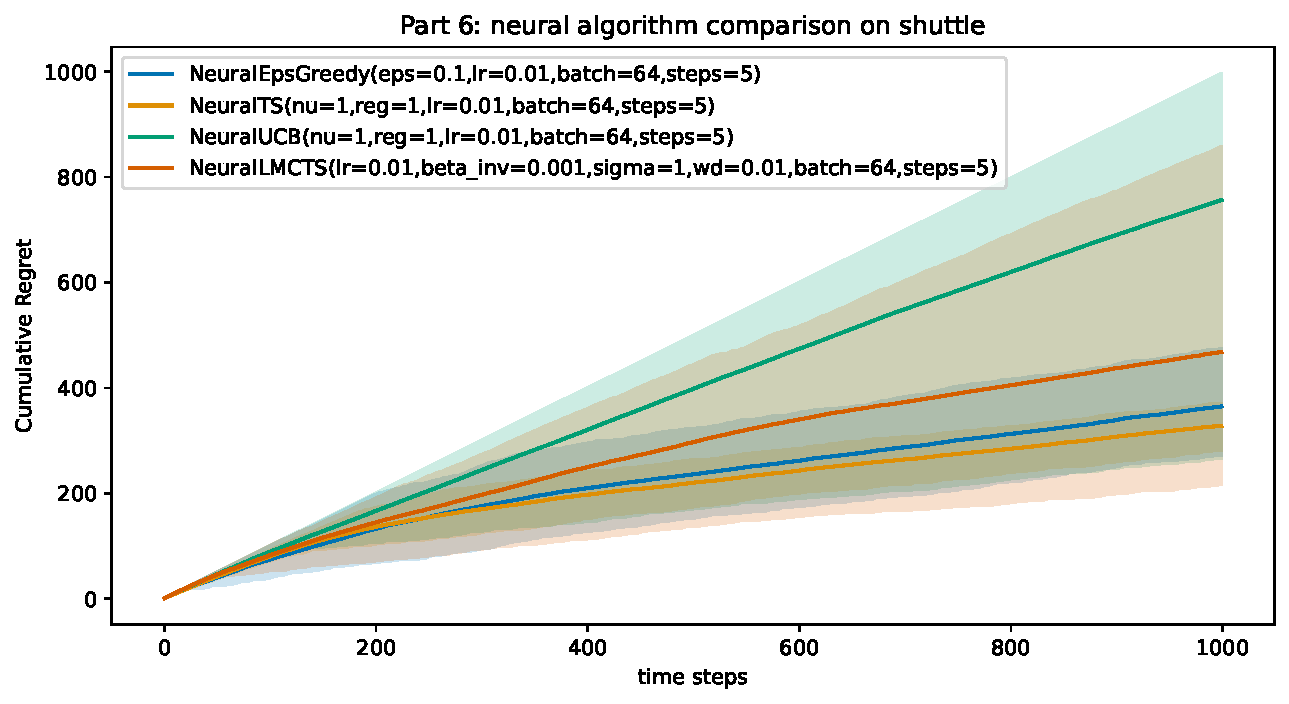
\includegraphics[width=0.96\linewidth]{../artifacts/full-20261101-1923/parts1-6/figures/cell_038_figure_010.pdf}
\caption{Cumulative regret in the fresh shuttle comparison.}
\label{fig:shuttle-final}
\end{figure}

\clearpage
\section*{Part 7A. Movie recommendations with an LLM}
\pdfbookmark[1]{Part 7A. Movie recommendations with an LLM}{part7A}
Qwen3.5-0.8B acted as a viewer and scored one selected movie without conversation history.
There were eight fixed movies. Role A preferred space science and engineering;
Role B preferred romantic musicals and accepted cartoons.
An integer score from zero to ten was divided by ten, perturbed by $N(0,0.1^2)$,
and clipped to $[0,1]$. Sampling used temperature $0.5$, top-$p=0.9$, and top-$k=20$.

Random, Greedy, $\epsilon$-greedy ($\epsilon=0.1$), and UCB were compared using seed 7001.
UCB tried each movie once and then used the bonus $\sqrt{2\log(t+1)/n_a}$.
Ties were broken randomly. Identical choices shared one fresh score within a round;
scores were not carried into later rounds. The roles used common random seeds.

$\epsilon$-greedy had the highest mean reward for both roles. UCB had lower means but much smaller variation between runs. Both favored The Martian for Role A and selected La La Land most often for Role B. $\epsilon$-greedy also selected Toy Story in 43.73\% of Role B rounds, consistent with that role accepting cartoons.

\begin{table}[H]
\centering
\small
\caption{Final cumulative movie rewards ($N=3$ per role).}
\label{tab:movies}
\begin{tabularx}{\linewidth}{@{}Xrr@{}}
\toprule
Policy & Role A & Role B \\
\midrule
Random & 490.09 $\pm$ 10.58 & 627.69 $\pm$ 9.41 \\
Greedy & 612.05 $\pm$ 273.43 & 565.43 $\pm$ 187.63 \\
$\epsilon$-greedy (0.1) & 786.68 $\pm$ 34.34 & 788.35 $\pm$ 18.56 \\
UCB & 718.46 $\pm$ 2.96 & 749.91 $\pm$ 6.33 \\
\bottomrule
\end{tabularx}
\end{table}

\begin{figure}[H]
\centering
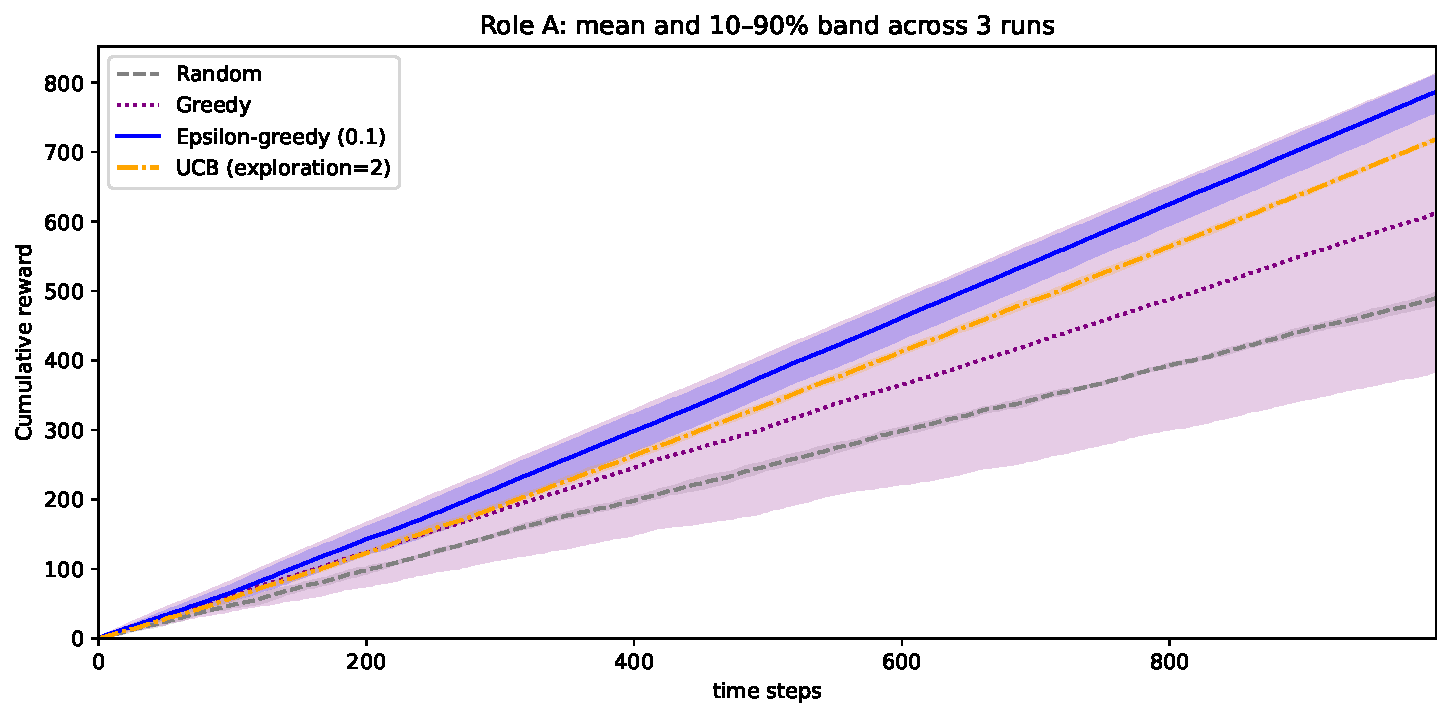
\includegraphics[width=0.96\linewidth]{../artifacts/full-20261101-1923/7a/figures/cell_052_figure_001.pdf}
\caption{Cumulative movie reward for Role A, who preferred space science.}
\label{fig:movie-a}
\end{figure}

\begin{figure}[H]
\centering
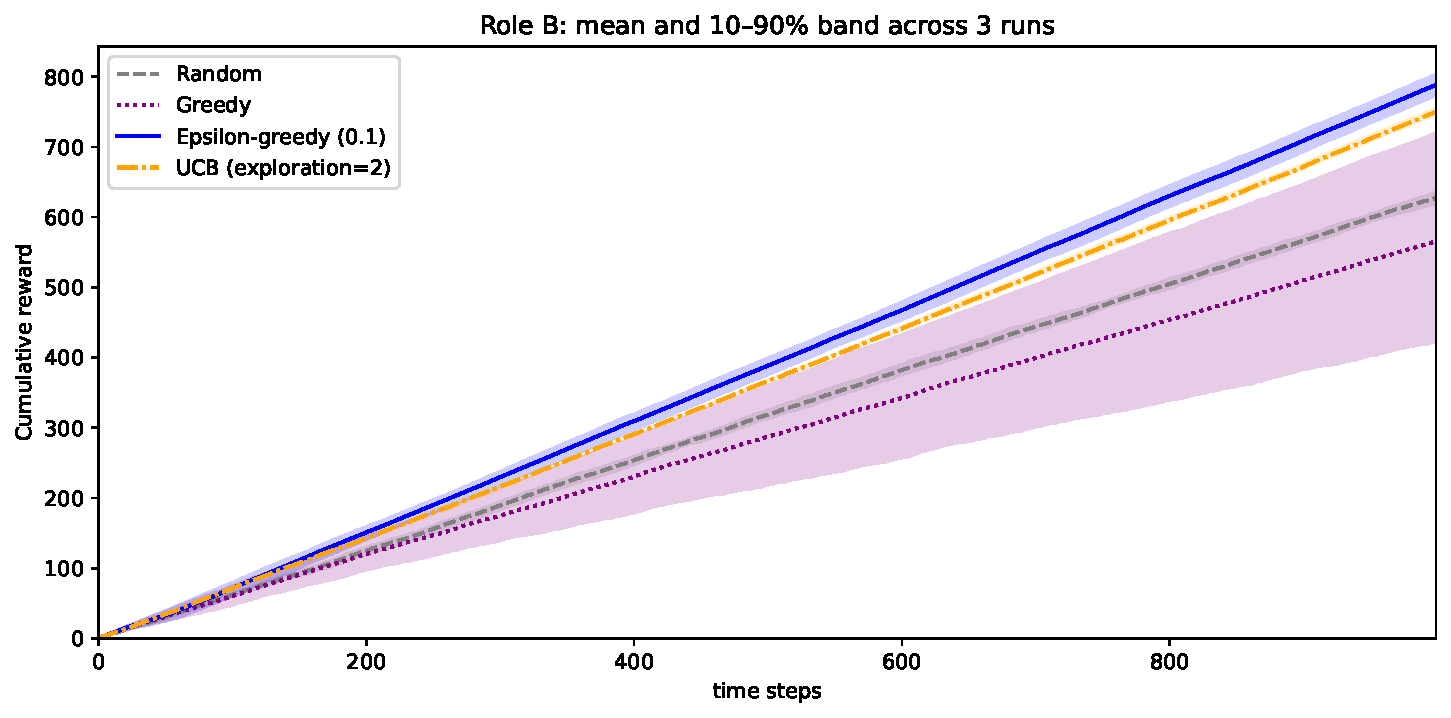
\includegraphics[width=0.96\linewidth]{../artifacts/full-20261101-1923/7a/figures/cell_056_figure_003.pdf}
\caption{Cumulative movie reward for Role B, who preferred romantic musicals.}
\label{fig:movie-b}
\end{figure}

Greedy's three-way tie comes from different runs, rather than balanced choices within a run. It selected Titanic, Ocean's Eleven, or The Martian for all 1000 rounds in one run each, under both roles. This dependence on the initial choice explains its high variability and its lower mean than Random for Role B. Random's most-selected movie reflects sampling rather than learning. No independent oracle established which movie had the highest expected reward.

\begin{table}[H]
\centering
\small
\caption{Most-selected movie and mean selection share for each policy. Greedy tied across runs.}
\label{tab:movie-choices}
\begin{tabularx}{\linewidth}{@{}Xrr@{}}
\toprule
Policy & Role A & Role B \\
\midrule
Random & Ocean's Eleven (14.30\%) & Ocean's Eleven (14.30\%) \\
Greedy & Three-way tie (33.33\% each) & Three-way tie (33.33\% each) \\
$\epsilon$-greedy (0.1) & The Martian (82.30\%) & La La Land (45.77\%) \\
UCB & The Martian (60.33\%) & La La Land (25.03\%) \\
\bottomrule
\end{tabularx}
\end{table}

\begin{figure}[H]
\centering
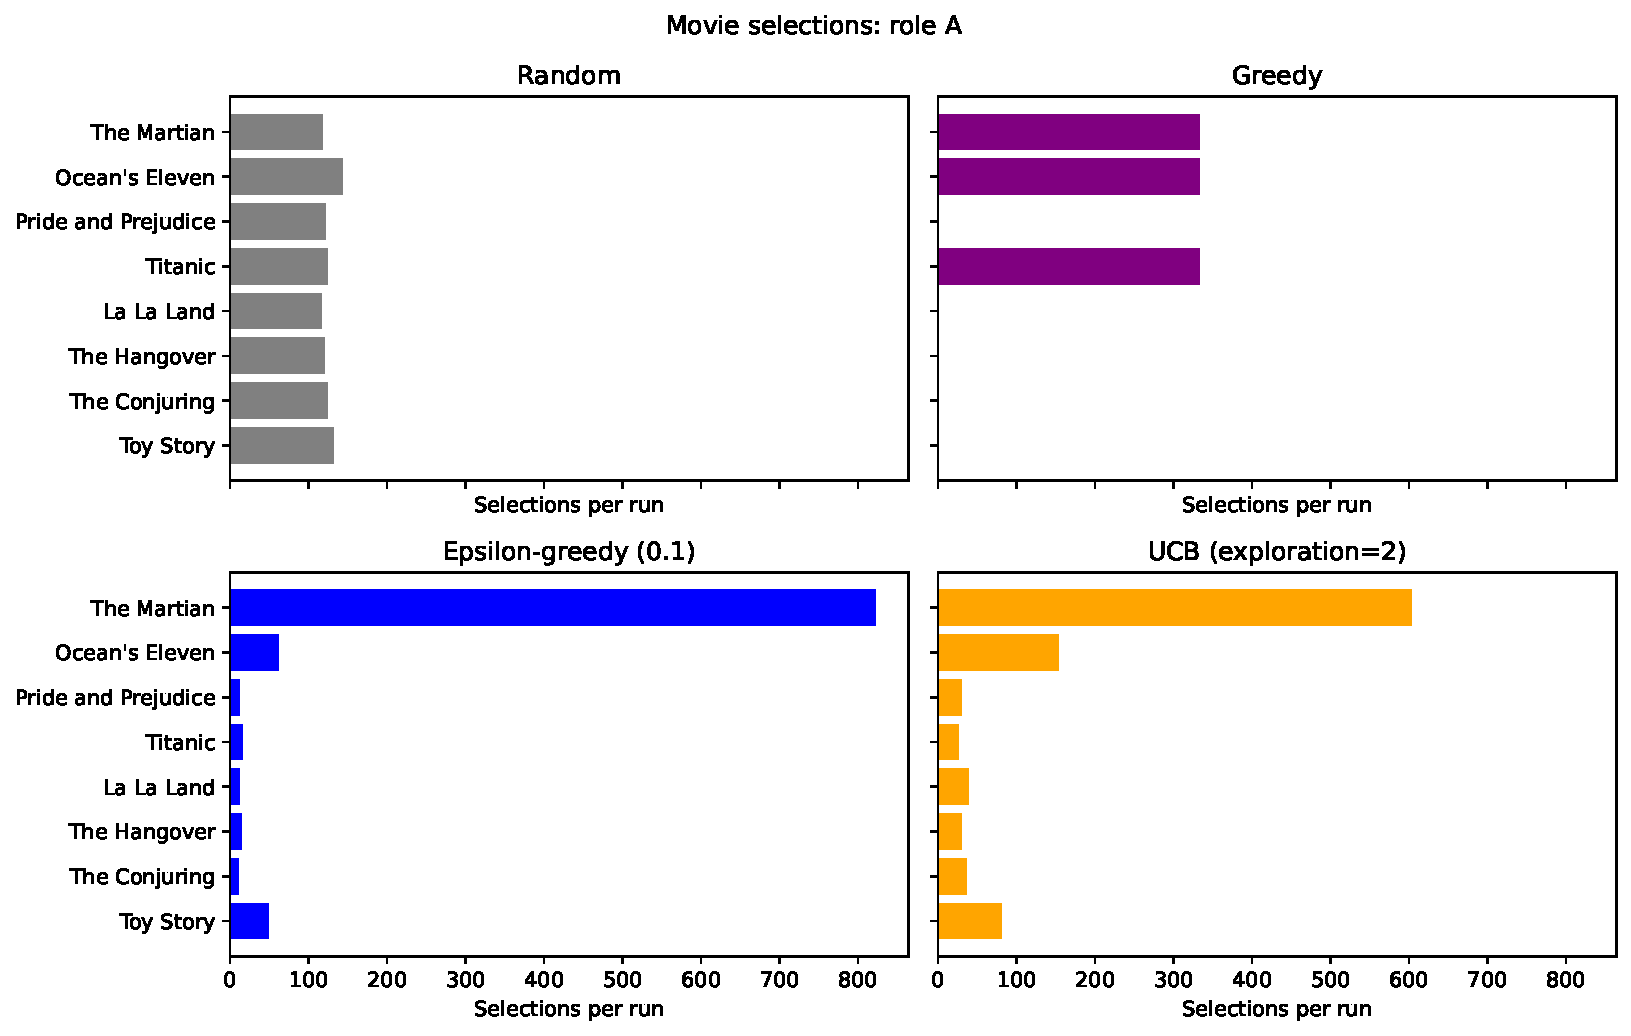
\includegraphics[width=0.96\linewidth]{../artifacts/full-20261101-1923/7a/figures/cell_053_figure_002.pdf}
\caption{Mean movie-selection counts per run for Role A.}
\label{fig:movie-count-a}
\end{figure}

\begin{figure}[H]
\centering
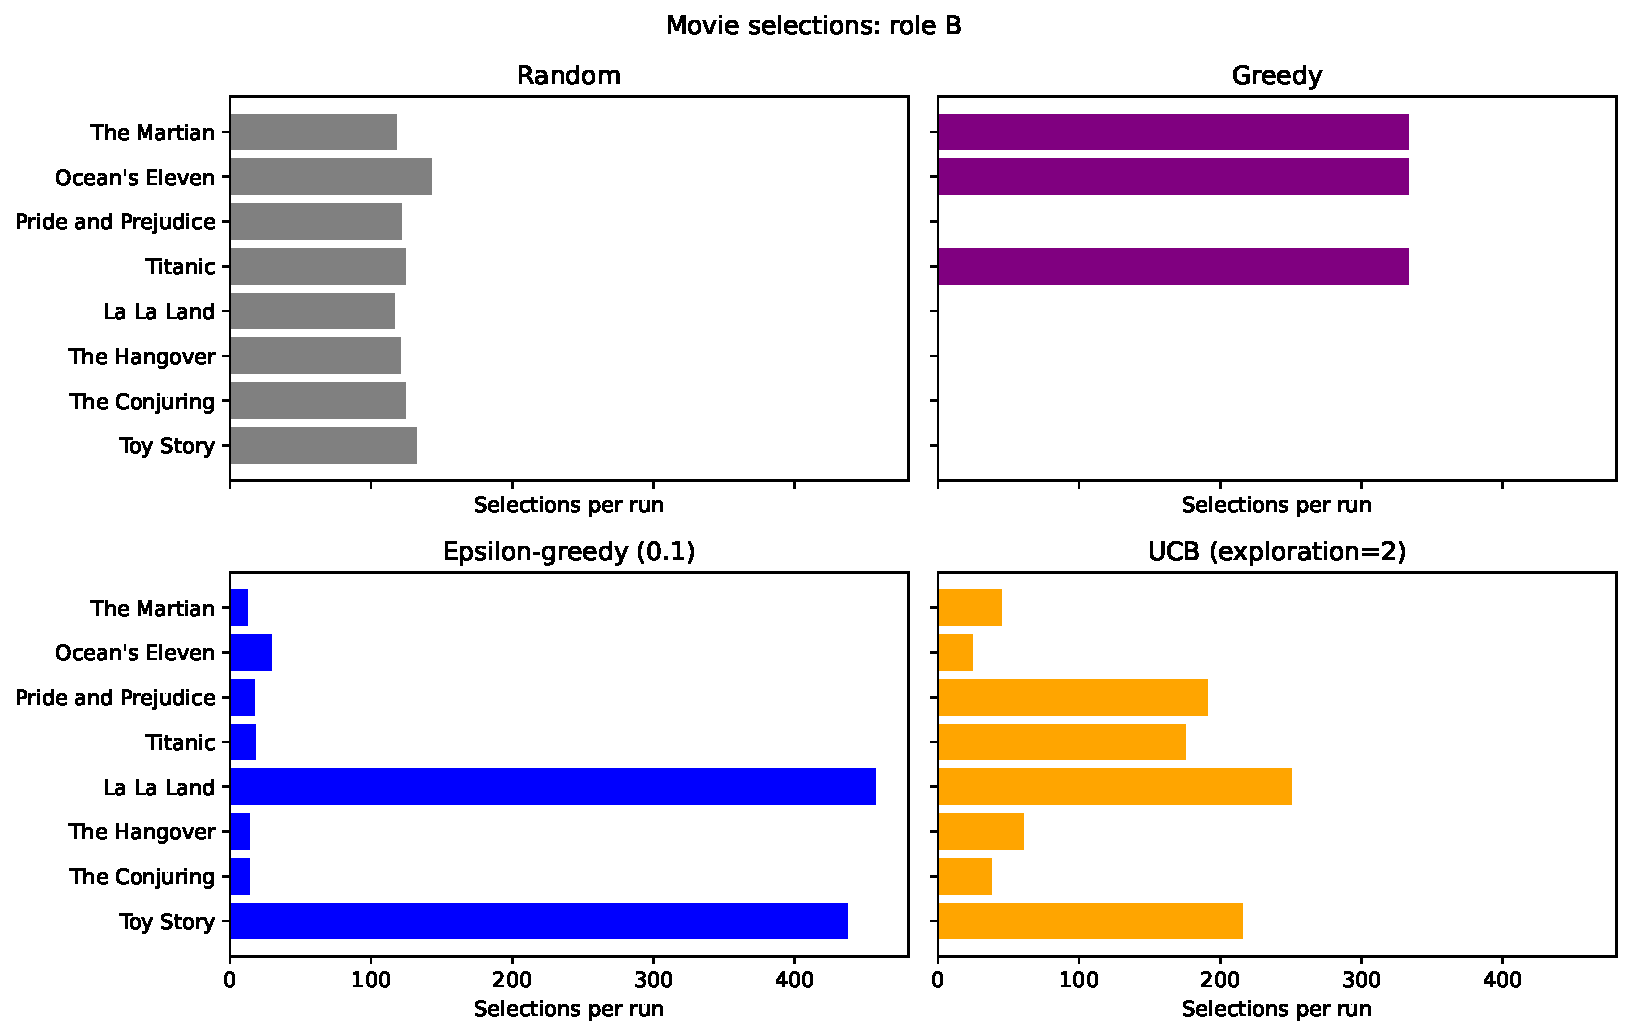
\includegraphics[width=0.96\linewidth]{../artifacts/full-20261101-1923/7a/figures/cell_057_figure_004.pdf}
\caption{Mean movie-selection counts per run for Role B.}
\label{fig:movie-count-b}
\end{figure}

\section*{Part 7B. ChatDoctor bandit with an LLM patient}
\pdfbookmark[1]{Part 7B. ChatDoctor bandit with an LLM patient}{part7B}
The candidate set contained five fixed ChatDoctor questions and 17 distinct responses
from \href{https://huggingface.co/datasets/TsinghuaC3I/UltraMedical-Preference}{UltraMedical-Preference}.
Qwen2.5-0.5B supplied last-token embeddings for each question-response pair.
A seed-42 random projection reduced these to 32 dimensions.
After normalization, centering, and PCA, 16 components were scaled by a common radius.
After adding an intercept, the features were divided by $\sqrt{2}$, producing 17-dimensional arm features.

Qwen3.5-0.8B returned a satisfaction score from zero to ten; reward was score divided by ten,
without added Gaussian noise. Sampling used temperature $0.3$, top-$p=0.9$, and top-$k=20$.
Profile A preferred plain main advice and a clear next step.
Profile B preferred detailed reasoning relevant to the reported symptoms.
Random, LinUCB ($\alpha=\lambda=1$), and LinTS ($\nu=\lambda=1$) used seed 7002.
Each learner maintained its own ridge estimate across questions.
Policies shared the question in each round and fresh scores for identical response choices.
The question schedules also matched between profiles.

LinUCB had the highest mean reward for both profiles, followed by LinTS. Its cumulative gains over Random were 45.70 for Profile A and 56.00 for Profile B. These correspond to gains of 0.0457 and 0.0560 per round.

Every policy received higher rewards under Profile B. This pattern is consistent with the available responses matching its preference for detailed explanations. However, changing the profile also changes the satisfaction criterion. These results do not isolate an answer-length effect or establish clinical quality.

The comparison covers five fixed questions and 17 responses, using fixed encoded/PCA features and matching A/B question schedules. The conclusions are limited to these responses, simulated preferences, model revisions, and seeds.

\begin{table}[H]
\centering
\small
\caption{Final cumulative satisfaction rewards ($N=3$ per profile).}
\label{tab:medical}
\begin{tabularx}{\linewidth}{@{}Xrr@{}}
\toprule
Policy & Profile A & Profile B \\
\midrule
Random & 756.87 $\pm$ 5.27 & 889.73 $\pm$ 5.98 \\
LinUCB & 802.57 $\pm$ 5.78 & 945.73 $\pm$ 3.91 \\
LinTS & 773.03 $\pm$ 2.62 & 916.67 $\pm$ 2.24 \\
\bottomrule
\end{tabularx}
\end{table}

\begin{figure}[H]
\centering
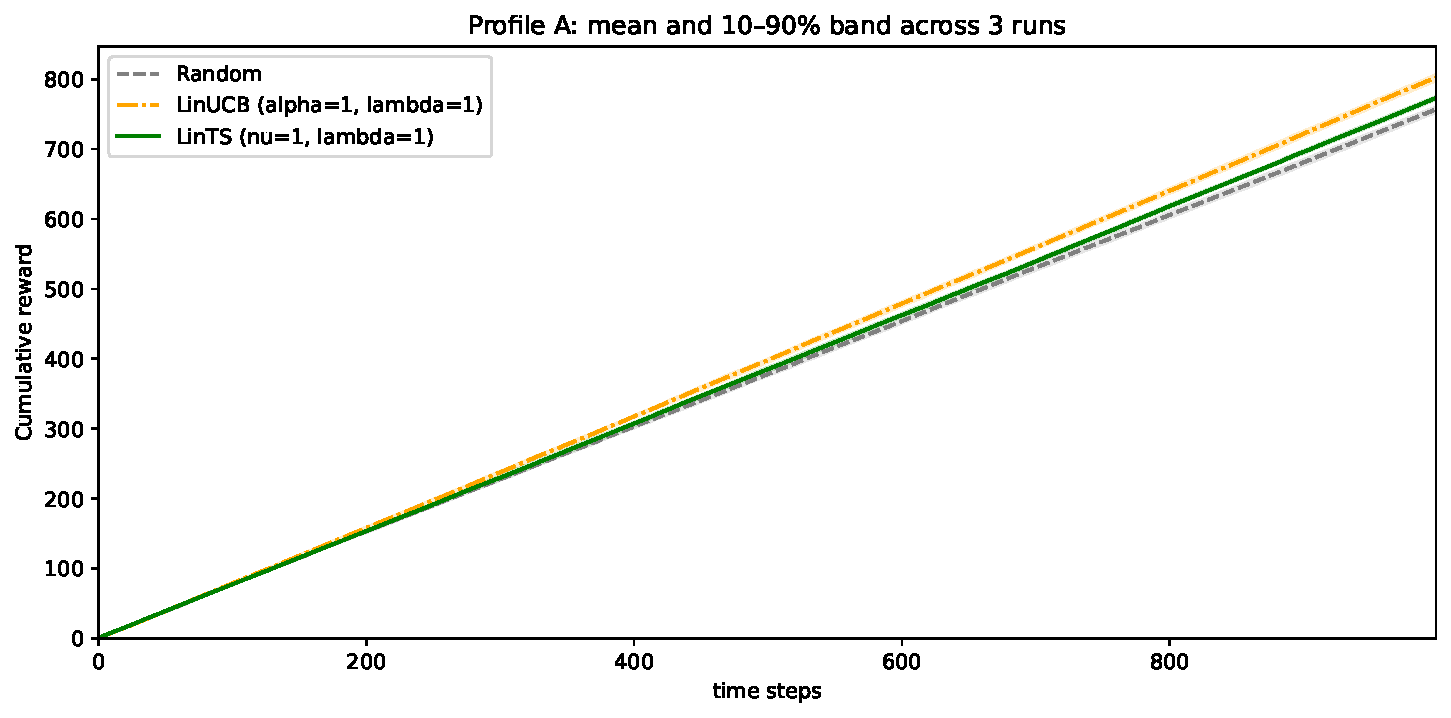
\includegraphics[width=0.96\linewidth]{../artifacts/full-20261101-1923/7b/figures/cell_072_figure_001.pdf}
\caption{Cumulative satisfaction reward for Profile A, who preferred plain advice.}
\label{fig:medical-a}
\end{figure}

\begin{figure}[H]
\centering
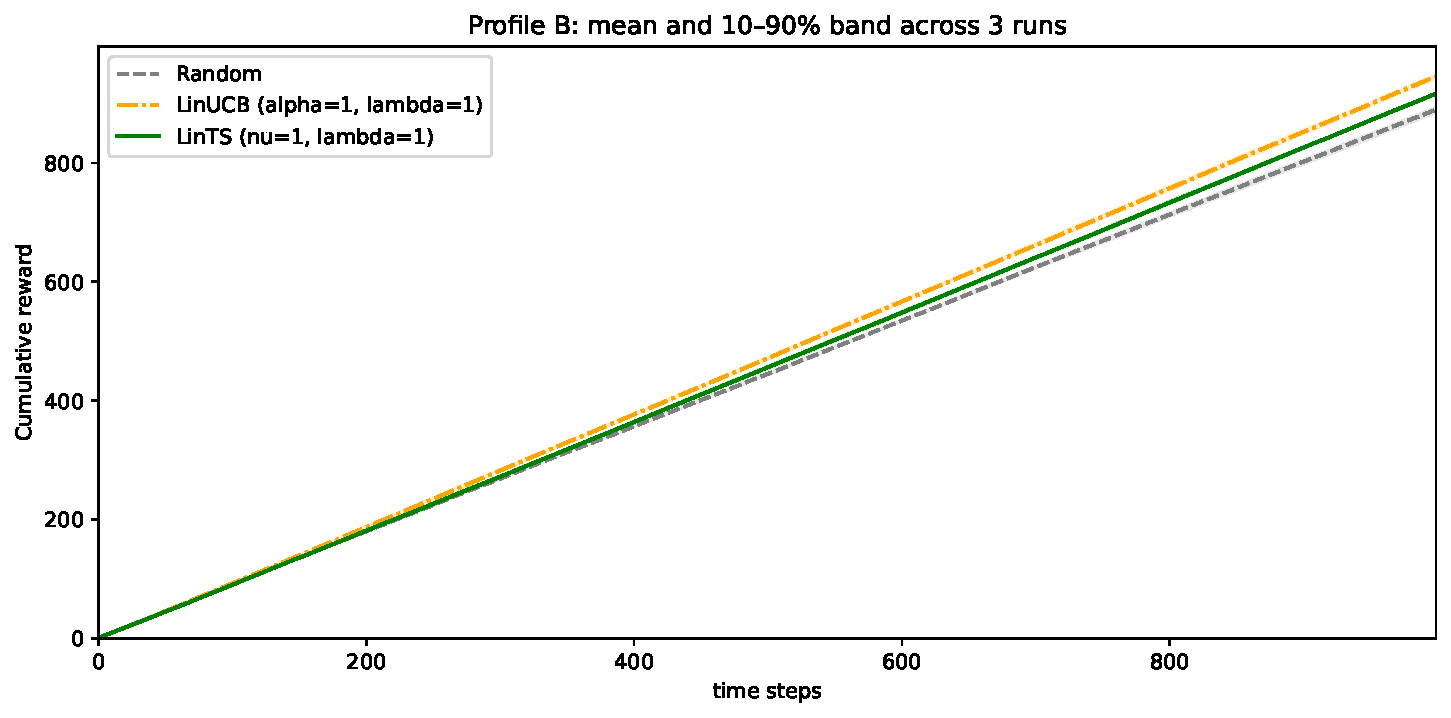
\includegraphics[width=0.96\linewidth]{../artifacts/full-20261101-1923/7b/figures/cell_075_figure_002.pdf}
\caption{Cumulative satisfaction reward for Profile B, who preferred detailed explanations.}
\label{fig:medical-b}
\end{figure}

\section*{Code and reproducibility}
The completed code is in \texttt{Experiments.ipynb}. Saved arrays, original figures,
and exact model revisions are recorded in the
\href{https://github.com/zhouhanqian1-sys/bandit-algorithms}{project repository}.
The scorer was Qwen3.5-0.8B (revision \texttt{2fc0636}); the encoder was
Qwen2.5-0.5B (\texttt{060db64}). The medical dataset revision was \texttt{761eb79}.
The experiments ran in the existing RL environment on one Duke DCC H200,
using Python 3.11.18 and PyTorch 2.10.0+cu128.
\end{document}
